\section{Introduction}
\label{introduction}



%%%%%%%%%%%%%%%%%%%%%%%%%%%%%%%%%%%%%%%%%%%%%%%%%%%%%%%%%%%%%%%%%%%%%%
%%%%%%%% Figure 1
%%%%%%%%%%%%%%%%%%%%%%%%%%%%%%%%%%%%%%%%%%%%%%%%%%%%%%%%%%%%%%%%%%%%%%

\begin{figure}[t]
\begin{center}
% \fbox{\rule{0pt}{2in} \rule{0.9\linewidth}{0pt}}
   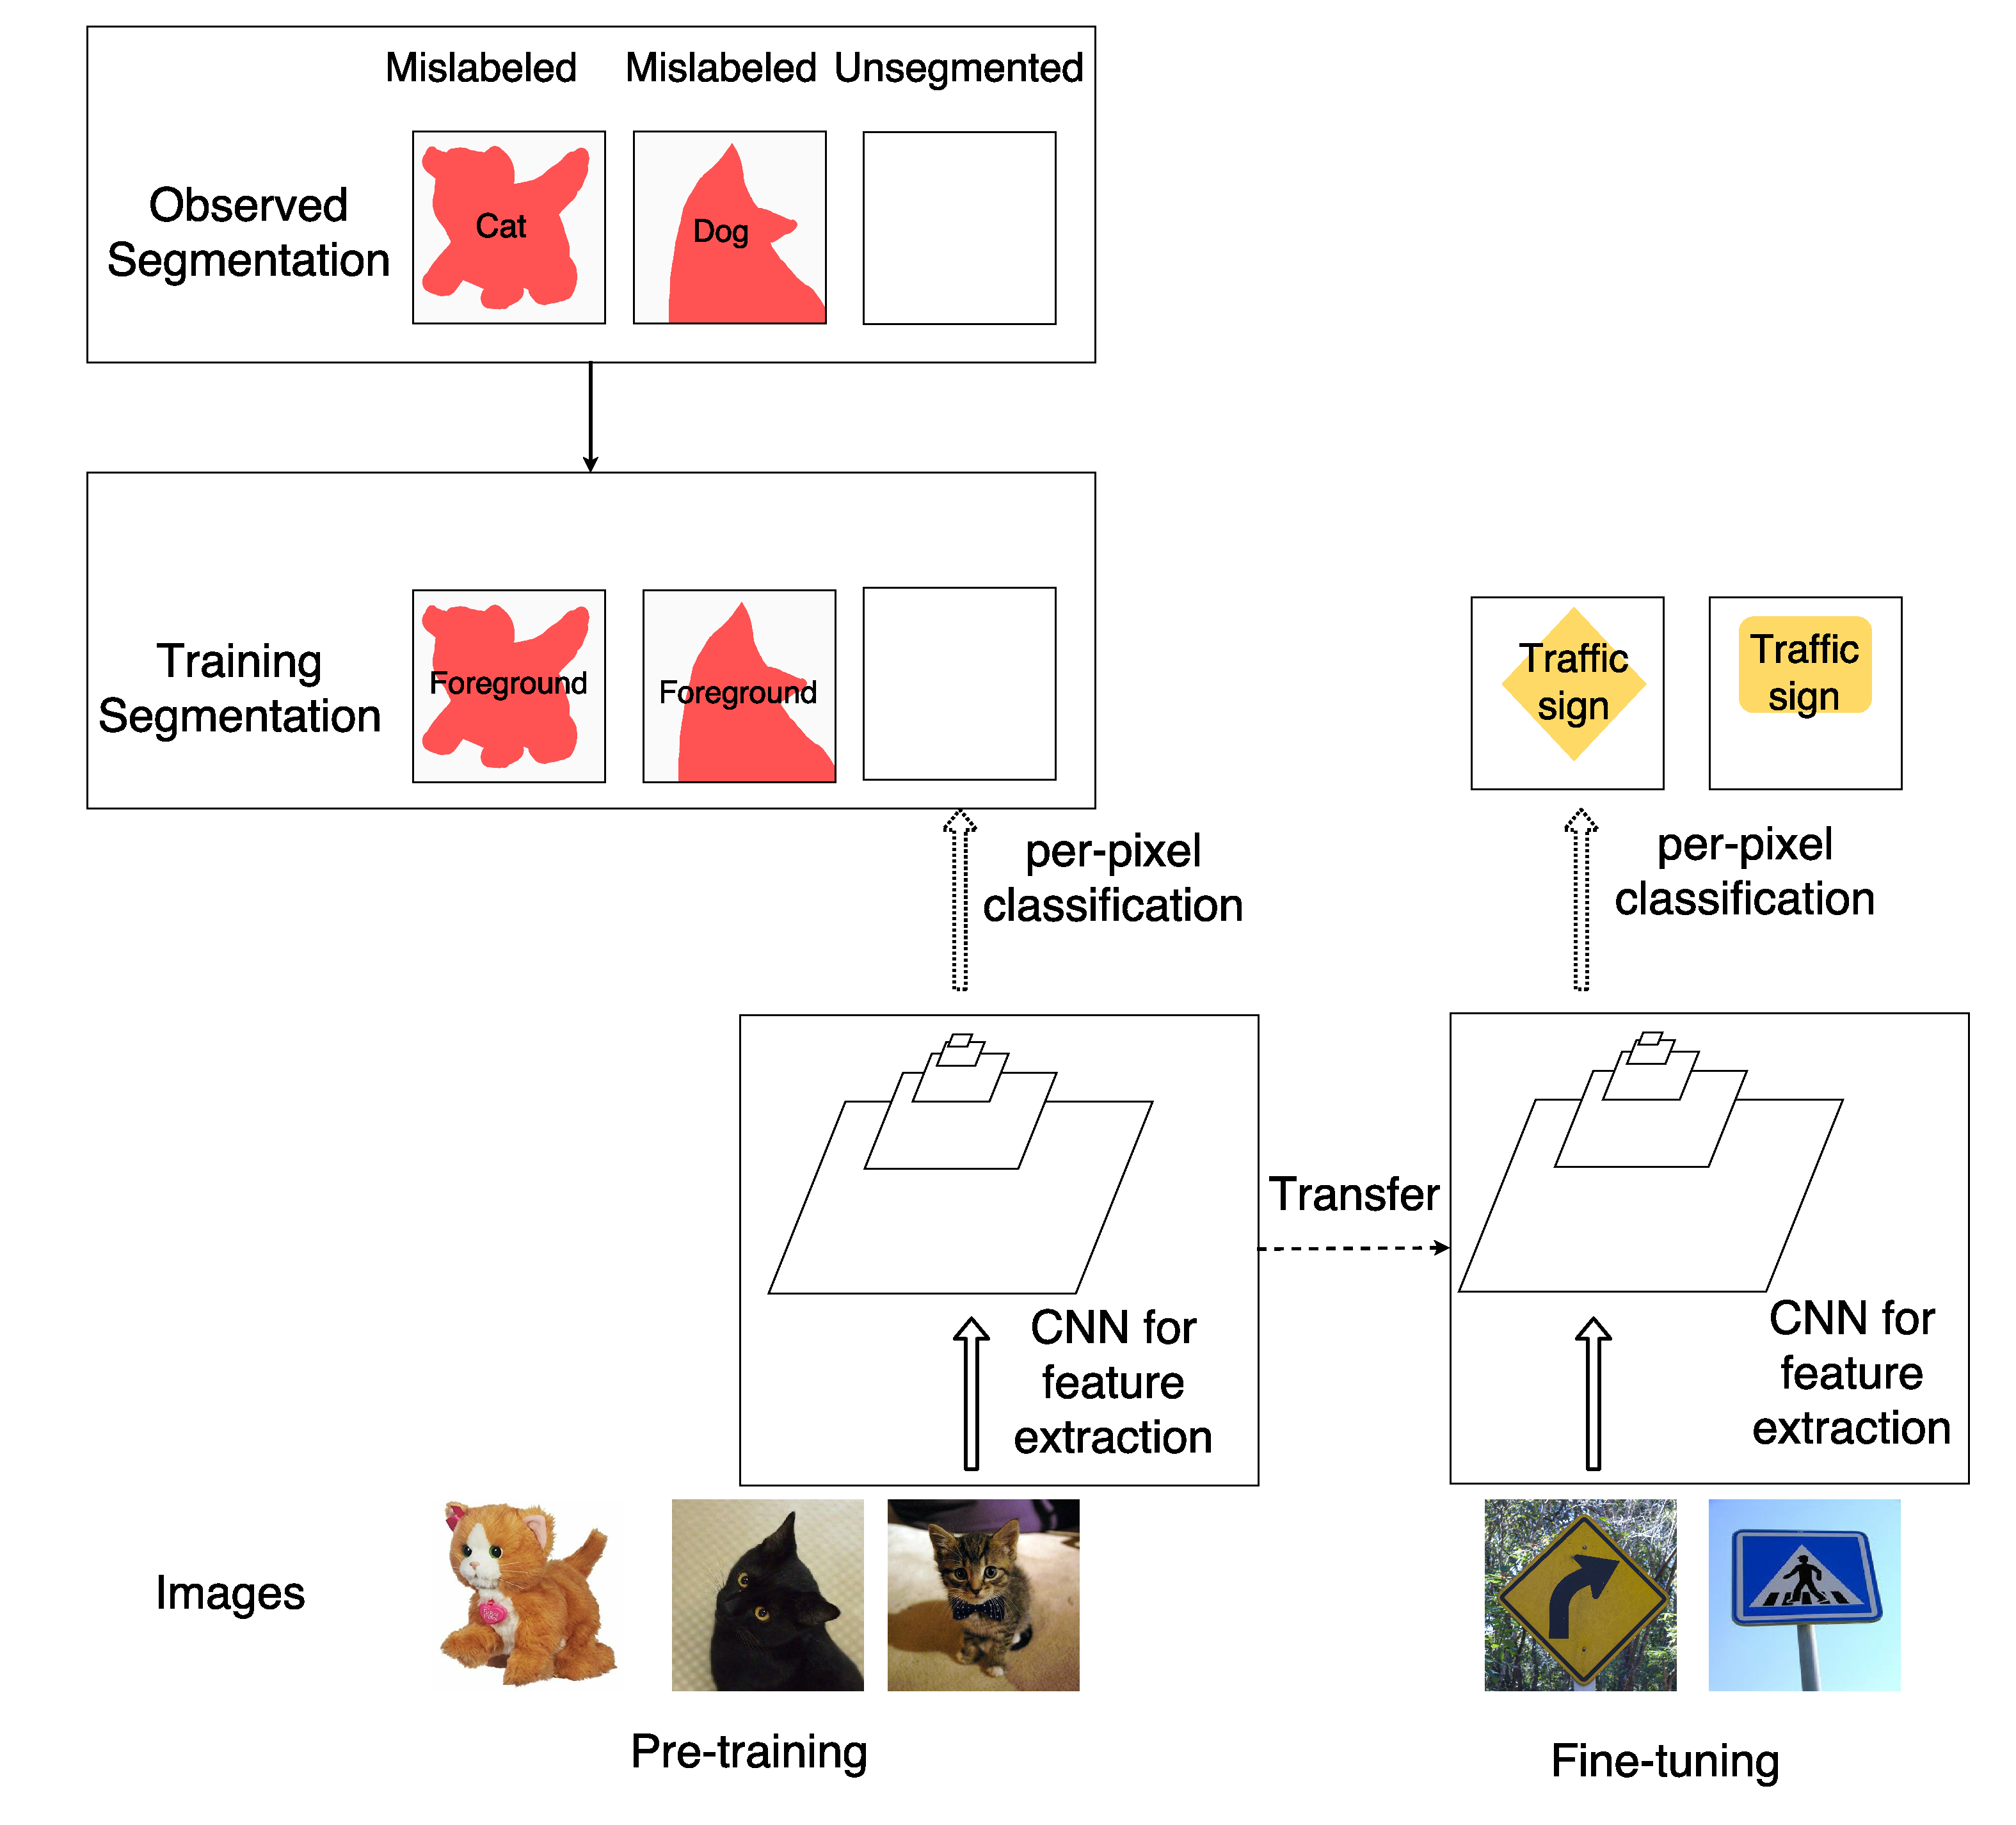
\includegraphics[width=1.05\linewidth]{img/figure1}
\end{center}
   \caption{
   Transferring feature extractor($g$) from convolutional neural networks for semantic segmentation pre-trained by potentially incomplete, mislabeled segmentations.
   }
\label{fig:figure1}
\end{figure}


%%%%%%%%%%%%%%%%%%%%%%%%%%%%%%%%%%%%%%%%%%%%%%%%%%%%%%%%%%%%%%%%%%%%%%
%%%%%%%% TEXT Why transfer learning?
%%%%%%%%%%%%%%%%%%%%%%%%%%%%%%%%%%%%%%%%%%%%%%%%%%%%%%%%%%%%%%%%%%%%%%

% \noindent \textit{Why transfer learning? \\
% Segmentation model benefits from transfer learning.
% \begin{itemize}
%   \item Success of CNN benefits from large-scale data whereas segmentation datasets are small
%   \item Collecting segmentation in one domain on a large scale can be difficult.
%   \item One can transfer pre-trained CNN model to train with limited training samples access.
% \end{itemize}
% }

The often limited availability of training samples motivates most state-or-the-art deep learning based segmentation models \cite{long2015fully,chen2016deeplab,he2017mask} to transfer convolutional neural network (CNN) models \cite{krizhevsky2012imagenet,simonyan2014very,szegedy2015going,he2016deep} trained on a subset of images from ImageNet.
% These ImageNet models \cite{krizhevsky2012imagenet,simonyan2014very,szegedy2015going,he2016deep} were originally trained for an object recognition task, the ILSVRC \cite{russakovsky2015imagenet} challenge, using around 1.2 million labeled images.
Compared to object recognition tasks, it is tougher to collect a dataset for semantic segmentation on a large scale.
The difficulty of obtaining manual segmentations is natural because it costs much more efforts for people to segment than to classify an image.
One of the largest segmentation datasets, Microsoft COCO2014 \cite{lin2014microsoft}, contains 123,287 images of 80 object categories, smaller in the number of images than the ILSRVC dataset by a factor of 10 approximately.
% the Pascal VOC2012 challenge \cite{everingham2015pascal} provides a segmentation dataset with only 9,993 segmented images for 20 object categories;
% The PASCAL-context Dataset \cite{mottaghi2014role} enriches the PASCAL VOC dataset by segmenting all 11,530 training images for 540 categories;
Transferring weights from the pre-trained ImageNet models can provide a segmentation performance boost in the limitation of lacking training samples, as reported in \cite{long2015fully} and adopted by \cite{chen2016deeplab,he2017mask}.

%%%%%%%%%%%%%%%%%%%%%%%%%%%%%%%%%%%%%%%%%%%%%%%%%%%%%%%%%%%%%%%%%%%%%%
%%%%%%%% TEXT Why pre-training with segmentation?
%%%%%%%%%%%%%%%%%%%%%%%%%%%%%%%%%%%%%%%%%%%%%%%%%%%%%%%%%%%%%%%%%%%%%%

% \noindent \textit{Why pre-training with segmentation? \\
% ImageNet models have limitations.
% \begin{itemize}
%   \item Disimilarity in domain of interest for training images
%   \item Architecture limitation of ImageNet models. (3D ConvNet)
% \end{itemize}
% }

However, it can be challenging to employ directly the ImageNet CNN models for semantic segmentation.
Firstly, the first layer of ImageNet models is not compatible with RGB-D images and 3D images like CT scans and MRI scans in 3D.
\cite{zheng2015conditional}.
Secondly, ImageNet models were originally trained with natural images at relatively low resolution.
In some domains of interest, images can be non-natural, such as aerial images, images from bird's eye view, and medical images;
In some other domains, images may have different lighting conditions or have a high resolution than the ImageNet ones.
Lastly, segmentation models do not necessarily follow the architecture design of classification models.
For example, the object recognition models pursue features invariance to better capture semantics regardless the variations in objects.
The result translation invariant and resolution-reduced features could reduce the localization accuracy which is not essential for object recognition but is critical for object segmentation. \cite{zheng2015conditional,chen2016deeplab}
This difference in requirements of features can result in different neural network architectures for segmentation models
Therefore, re-training ImageNet models, or even pre-train models from scratch in particular cases, using a segmentation dataset similar to but different from the one of interest can be more beneficial than employing ImageNet models directly.

% \footnote{The KITTI Vision Benchmark Suite http://www.cvlibs.net/datasets/kitti/}

%%%%%%%% ? Deeplab https://arxiv.org/pdf/1606.00915.pdf
%%%%%%%% In particular we consider three challenges in the application of DCNNs to semantic image segmentation: (1) reduced feature resolution, (2) existence of objects at multiple scales, and (3) reduced localization accuracy due to DCNN invariance.
%%%%%%%% ? CRFasRNN http://www.robots.ox.ac.uk/~szheng/papers/CRFasRNN.pdf
%%%%%%%% Firstly, traditionalCNNs have convolutional filters with large receptivefields and hence produce coarse outputs when restructured to produce pixel-level labels [37]
%%%%%%%% Secondly, CNNs lack smoothness constraints that encourage label agreement between similar pixels, and spatial and appearance consistency of the labelling output


%%%%%%%%%%%%%%%%%%%%%%%%%%%%%%%%%%%%%%%%%%%%%%%%%%%%%%%%%%%%%%%%%%%%%%
%%%%%%%% TEXT Why labels are noisy?
%%%%%%%%%%%%%%%%%%%%%%%%%%%%%%%%%%%%%%%%%%%%%%%%%%%%%%%%%%%%%%%%%%%%%%

% \noindent
% \textit{Why labels are noisy?
% \begin{itemize}
%   \item Crowd-sourcing data is noisy by nature.
%   \item ``gold standard'' itself can be ambiguous.
%   \item There exists free available noisy segmentation datasets
% \end{itemize}
% }

The segmentation datasets for pre-training may contain label noises.
The use of the crowd-sourcing platform like Mechanical Turk is common nowadays to collect annotations on a large-scale.
It is natural for crowd-sourcing workers to make mistakes as a result of lack of expertise, inherent ambiguity of tasks or unconscious bias.
Enormous efforts are required, according to  \cite{lin2014microsoft,everingham2015pascal}, to ensure the correctness of segmentations.
%A slight decrease in the percentage of segmentation errors, such as from 1\% to 0\%, may require extraordinary extra efforts due to the difficulty of identifying errors.
If not requiring ``gold standard'' segmentations for training, the efforts saved for correctness can be made to segment more images for a larger dataset.
%In some domains, for example, medical imaging, the ``gold standard'' itself can be ambiguous and cause disagreements among experts.
% \footnote{TODO M: But that's OK or not?  This is what probabilities solve...}
Besides,  some labels other than the manual ones may be freely available for particular tasks.
But these labels often contain structural noises depending on the way they were created.
For example, digital maps, like OpenStreetMap, can be used to segment aerial images.
Segmentations constructed from the maps could suffer from incompleteness as well as registration problems. \cite{mnih2012learning}
% Besides, Pl@ntNet\footnote{https://identify.plantnet-project.org/}, a crowdsourcing platform, provide millions of images of plants and corresponding labels which may or may not be correct.

%%%%%%%%%%%%%%%%%%%%%%%%%%%%%%%%%%%%%%%%%%%%%%%%%%%%%%%%%%%%%%%%%%%%%%
%%%%%%%% TEXT What types of noises exist and motivate them?
%%%%%%%%%%%%%%%%%%%%%%%%%%%%%%%%%%%%%%%%%%%%%%%%%%%%%%%%%%%%%%%%%%%%%%

% \noindent \textit{What types of noises exist and motivate them?
% \begin{itemize}
%   \item Inexaustive segmentation
%   \item Misclassification
%   \item False segmentations
% \end{itemize}
% }

% \paragraph{Segmentation noises}
Noises of different kinds can exist in segmentation labels. %inexhaustive segmentation, misclassification of segments, false segmentation, over-segmenting, under-segmenting, etc.
In particular, we consider mislabeling errors for the whole segment, assuming the outline of objects is always correct.
We categorized object mislabelling into three categories: inexhaustive segmentation, misclassification, and false segmentation.
\textbf{Misclassification} of objects from one category to another exist occasionally even for well-annotated datasets.
For example, the Microsoft COCO dataset \cite{lin2014microsoft} contains some misclassified bears and teddy bears even though annotators were asked to segment only one category at a time;
\textbf{Inexhaustive segmentation} means that there exist objects left unsegmented.
A typical scenario where incomplete segmentation emerges is to segment images containing massive amounts of objects of the same kind, e.g., a flock of sheep or a pile of products;
\textbf{False segmentation} denotes that semantically meaningful objects from an undefined category are wrongly segmented, as objects of interest.
It may occur due to the unclear definition of categories, visual similarities between objects, etc.


%%%%%%%%%%%%%%%%%%%%%%%%%%%%%%%%%%%%%%%%%%%%%%%%%%%%%%%%%%%%%%%%%%%%%%
%%%%%%%% TEXT Why binarizing classes?
%%%%%%%%%%%%%%%%%%%%%%%%%%%%%%%%%%%%%%%%%%%%%%%%%%%%%%%%%%%%%%%%%%%%%%

We simulated these three types of noises with a well-annotated dataset separately and studied their influences to the trained weights transferability in a transfer learning setup demonstrated in Figure \ref{fig:figure1}.
Ideally, noises in the pre-training datasets should not significantly affect transferring the learned model to another dataset.
But if negative influences introduced by label noises are remarkable, methods of compensating the noises become necessary.

% \noindent \textit{Why binarizing classes?}

Supposing misclassification had a negative influence on feature transferability, as we will show in Section \ref{subsec:robustness}, simply segmenting the foreground objects against the background can produce correct labels for misclassified objects.
It can be regarded as converting precise but potentially inaccurate labels to accurate but imprecise labels.
Training transferable features may not require as precise supervision as training classifiers because transferability of features are correlated to feature generality, i.e., if they are independent of particular categories \cite{yosinski2014transferable}.
Besides, Jain et al. \cite{jain2017pixel} proved the possibility of training a fully convolutional network to generate foreground segmentations.
Surprisingly, the model trained on over 1 million images generalizes well to object categories not included in the training.
Therefore, we argue that it should be possible to learn transferable representations by segmenting foreground and background in images.

% Deprecated examples
% There are a few examples proved the possibility of training binary object detection/segmentation:
% Ren et al. \cite{ren2015faster} trained CNN model to perform binary classification for region of interest proposals;
% He et al. \cite{he2017mask} trained binary segmentation in addition to object detection for instance-aware segmentation;

%%%%%%%%%%%%%%%%%%%%%%%%%%%%%%%%%%%%%%%%%%%%%%%%%%%%%%%%%%%%%%%%%%%%%%
%%%%%%%% TEXT Why PU learning
%%%%%%%%%%%%%%%%%%%%%%%%%%%%%%%%%%%%%%%%%%%%%%%%%%%%%%%%%%%%%%%%%%%%%%

If we consider inexhaustive segmentation only, the problem becomes similar to a so-called \textit{positive and unlabelled learning} (PU learning) setup \cite{li2005learning}.
In the positive and unlabeled learning setup, the training dataset has two sets of examples: a \textit{positive (P) set}, containing only positive examples, and an \textit{unlabeled (U) set}, containing a mix of positive or negative examples.
The P set in an incompletely segmented dataset is comprised of segmented pixels while the rest of the pixels construct the U set.
The main characteristic of the U set is no easy way to generate reliable negative labels out of it.
Semi-supervised learning techniques are consequently not applicable as a result of the absence of negative training samples.
The set of background pixels containing unsegmented objects can fulfill this property of U set.
Learning to segment objects in the presence of inexhaustive segmentation can be therefore considered as a learning problem with only positive examples and unlabeled examples.
In this work, we treat the unlabeled set as a set of examples with noisy negative labels and modify the loss for the negative class accordingly, following a branch of previous studies for PU learning as discussed in Section \ref{sec:related}.
% We then proposed a sigmoidal loss for negative samples based on the idea of not over-punishing confident, positive predictions when learning in the presence of mislabeled positive samples.

% \noindent

% Experiments in Section \ref{subsec:robustness} indicates that inexhaustive segmentation can have significant negative influences on feature transferability.
% Besides, including mis-segmented objects for training can aggravate the inexhaustive segmentation problem.
% For example, the existence a mis-segmented toy dog does not mean that every toy dogs are mis-segmented.
% The other unsegmented toy dogs then become a source of inexhaustive segmentation and lead to worse fine-tuning performance as we discovered in Section \ref{sec:experiments}.
% Method to compensate inexhaustive segmentation is therefore necessary to train better transferable representation.

%%%%%%%%%%%%%%%%%%%%%%%%%%%%%%%%%%%%%%%%%%%%%%%%%%%%%%%%%%%%%%%%%%%%%%
%%%%%%%% TEXT Main contributions
%%%%%%%%%%%%%%%%%%%%%%%%%%%%%%%%%%%%%%%%%%%%%%%%%%%%%%%%%%%%%%%%%%%%%%

The main topics discussed in this thesis are:
\begin{enumerate}
  \item How mislabeling of segmentations influences feature transferability of CNN models for semantic segmentation?
  \item Compared to the inaccuracy of pre-training labels, how impreciseness of labels affects feature transferability?
  \item How to modify the loss function to achieve better pre-training and fine-tuning performances in the presence of incomplete segmentations?
\end{enumerate}

%%%%%%%%%%%%%%%%%%%%%%%%%%%%%%%%%%%%%%%%%%%%%%%%%%%%%%%%%%%%%%%%%%%%%%
%%%%%%%% TEXT Table of contents
%%%%%%%%%%%%%%%%%%%%%%%%%%%%%%%%%%%%%%%%%%%%%%%%%%%%%%%%%%%%%%%%%%%%%%

The rest of this thesis is organized as follows:
In the next section, we summarize related works.
 % in areas of transfer learning, deep learning with noisy labels and PU learning.
In Section \ref{sec:robustness} we formulate the problem of transferring segmentation models pre-trained with noisy segmentations, and how to synthesize the three types segmentation noises.
We introduce a sigmoidal loss for the negative class to compensate noisy negative labels in Section \ref{sec:pulearning}.
Experiments in Section \ref{subsec:robustness} was designed to study the influences of inexhaustive segmentations, misclassification and false segmentation separately.
The proposed sigmoidal loss, together with the class-weighted loss and a modified hard bootstrapping loss, is evaluated in simulated PU learning setups in Section \ref{subsec:pulearning}.
Discussions are presented in Section \ref{sec:discussion} and conclusions are summarized in Section \ref{sec:conclusion}.
%Features learned by predicting the pixel objectness with inexaustive annotations were then validated with experiments described in Section \ref{sec:discussion}.
